\chapter{Results and Discussion}\label{chapter:results}
This chapter includes presentation and analysis of the results obtained in this thesis. Section \ref{section:parameter settings} presents results from testing different parameter settings for the genetic algorithm, and briefly discusses each results. Section \ref{section:results} presents the main results obtained when running the different population distributed genetic algorithms. Section \ref{section:discussion} contains a discussion and comparison of the results obtained in section \ref{section:results}.


\section{Parameter settings}\label{section:parameter settings}
Parameter settings are crucial for obtaining good results with the genetic algorithm. In order to find the right settings, simulations were run to find the best adult selection method, parent selection method, crossover method, crossover rate and mutation rate for the given problem. Even though it would take much shorter time and less effort to test these settings on a toy problem such as One Max, the decision was made to test them on the real problem. The reason behind this decision is that different settings might work better on different problems and the nature of the wind farm layout optimization problem is unique because of the importance of the wind turbine positions relative to each other. It is important to note that even though effort was made to find good settings for the genetic algorithm,  it is impossible to obtain the optimal ones. Just imagine trying the test every single value for the continuous parameter crossover rate against every possible value of each of the other settings, just that would be impossible! Therefore, the values that are tested for each parameter setting is largely tested against values that are based on the authors previous experience with genetic algorithm and values close to those.\\

\begin{table}
\centering
\caption{Values kept fixed while one by one was changed in order to find the best settings for the wind farm layout optimization problem.}
\label{table:fixed settings}
\begin{tabular}{l|l}
\textbf{Parameter} & \textbf{Value} \\ 
\hline 
Wind scenario & 00.xml \\ 
Evaluator & KusiakLayoutEvaluator \\ 
Population size & 100 \\  
Generations & 100 \\ 
Elitism & true \\  
Flip mutation rate & 0.01 \\ 
Inversion mutation rate & 0.0 \\ 
Interchange mutation rate & 0.0 \\ 
Parent selection & Tournament selection \\ 
Tournament size & 5 \\ 
Epsilon & 0.0 \\  
Crossover method & Uniform crossover \\ 
Crossover rate & 0.9 \\ 
\end{tabular} 
\end{table}

\noindent For each simulation one of the parameters were tested while the others were kept fixed as shown in table \ref{table:fixed settings}. As can be seen in this table, other settings such as wind scenario, population size, number of generations, whether elitism should be used and mutation rate for interchange mutation and inversion mutation could also be tested, but since evaluation of each farm takes a lot of time, even on an 8 core computer running in parallel, simulations are not run to set these values. These settings are set using the authors previous experience and educated guessing. Testing different parameters on a single wind scenario might lead to values that are tailored for the given scenario and that are not as well suited for some of the others. However, there is no time to test each value for every single wind scenario, and this should not make that much of a difference. Population size is a value that influence the performance of the genetic algorithm largely. Greater population size often leads to better performance since more solutions increase the probability of finding the global optimal solution. The population size was set to 100 for two reasons. First of all, a population size of 100 is large enough so that many different solutions are explored. Second when the population size is kept at 100, the adult selection method ''Overproduction'' will produce twice as many children, so that 200 individuals has to be evaluated for each generation something that will double the evaluation time, the step that already is the bottleneck of the algorithm. The number of generations was kept at 100 for each run, evaluating each population for 100 generations takes time and it the main reason why the algorithm were not run for more generations, however, as can be seen on the graphs in the sections below the fitness looks like it is starting to flat out after a 100 generations indicating that a 100 generations are sufficient for the purpose of setting the parameter values. Elitism was set to true for every run without testing, meaning that the best individual of each generation will survive. This decision is based on the authors previous experience with genetic algorithm where experiments has shown that elitism leads to better results because the best individual is not lost due to coincidences. Different mutation methods were implemented for the genetic algorithm, but only the flip mutation rate was tested to find the best value. Usually, flip mutation is the only mutation method used with genetic algorithms and it is therefore also used as the main for of mutation in this thesis. Inversion mutation and interchange mutation are implemented, but they will only happen seldom to introduce more randomness to the algorithm. In the main simulations, they will be assigned extremely low probabilities so that their occurrence is so rare that they will introduce too much randomness, but hopefully make occasional ''jumps'' to different solutions spaces so that the algorithm do not get completely stuck in a local optimal solution. 


\subsection{Adult Selection}
Figure \ref{figure:adult selection methods} shows the results of running the genetic algorithm with the different adult selection methods. Figure \ref{figure:full generational replacement}, \ref{figure:generational mixing}, and \ref{figure:overproduction} shows the results for full generational replacement, generational mixing and overproduction respectively. As can be seen in the figures, full generational replacement ends up with an average best fitness of \textcolor{red}{average of best fitness}, generational mixing with an average best fitness of \textcolor{red}{average of best fitness}, and overproduction with an average best fitness of \textcolor{red}{average of best fitness}. These results are as expected. Note that generational mixing could never do worse than full generational replacement. If the results of reproduction leads to a population of individuals with strictly better fitness, generational mixing will replace the entire previous generation with the new one, as full generational replacement. However, if the new generation produces individuals with worse fitness than some of the individuals in the previous generation these old individuals will be kept instead, making sure that the new population has equal or better fitness than the previous one. Overproduction does not provide the same ''newer worst'' \textcolor{red}{Check word!} guarantee, however, as shown in figure \ref{figure:overproduction} it still outperforms generational mixing. Even though overproduction wipes out the entire previous population, it generates twice as many children at the reproduction step so its probability of getting it right is doubled. 


\begin{figure}[h!]
    \centering
    \begin{subfigure}[b]{0.31\textwidth}
        \includegraphics[width=\textwidth]{images/plots/"adult selection"/"full generational replacement"}
        \caption{}
        \hfill
        \label{plot:full generational replacement}
    \end{subfigure}
    ~
    \begin{subfigure}[b]{0.31\textwidth}
        \includegraphics[width=\textwidth]{images/plots/"adult selection"/"generational mixing"}
        \caption{}
        \hfill
        \label{plot:generational mixing}
    \end{subfigure}
    ~
    \begin{subfigure}[b]{0.31\textwidth}
        \includegraphics[width=\textwidth]{images/plots/"adult selection"/"overproduction"}
        \caption{}
        \hfill
        \label{plot:overproduction}
    \end{subfigure}
    \caption{Adult selection methods: (a) Full generational replacement, (b) generational mixing and (c) overproduction averaged over 10 runs.}
    \label{plot:adult selection methods}
\end{figure}


\subsection{Parent Selection}


\begin{figure}[h!]
    \centering
    \begin{subfigure}[b]{0.31\textwidth}
        \includegraphics[width=\textwidth]{images/plots/"parent selection"/"roulette wheel"}
        \caption{}
        \hfill
        \label{plot:roulette wheel}
    \end{subfigure}
    ~
    \begin{subfigure}[b]{0.31\textwidth}
        \includegraphics[width=\textwidth]{images/plots/"parent selection"/"tournament size 5"}
        \caption{}
        \hfill
        \label{plot:tournament size 5}
    \end{subfigure}
    ~
       \begin{subfigure}[b]{0.31\textwidth}
        \includegraphics[width=\textwidth]{images/plots/"parent selection"/"tournament size 10"}
        \caption{}
        \hfill
        \label{plot:tournament size 10}
    \end{subfigure}
    ~
       \begin{subfigure}[b]{0.31\textwidth}
        \includegraphics[width=\textwidth]{images/plots/"parent selection"/"tournament size 15"}
        \caption{}
        \hfill
        \label{plot:tournament size 15}
    \end{subfigure}
    ~
       \begin{subfigure}[b]{0.31\textwidth}
        \includegraphics[width=\textwidth]{images/plots/"parent selection"/"tournament size 20"}
        \caption{}
        \hfill
        \label{plot:tournament size 20}
    \end{subfigure}
    ~
    \begin{subfigure}[b]{0.31\textwidth}
        \includegraphics[width=\textwidth]{images/plots/"parent selection"/"tournament size 25"}
        \caption{}
        \hfill
        \label{plot:tournament size 25}
    \end{subfigure}
    \caption{Parent selection methods: (a) Roulette wheel, (b) Tournament selection averaged over 10 runs, tournament size 5 (c) tournament selection, tournament size 10, (d) tournament selection, tournament size 15, (e) tournament selection, tournaments size 20, and (f) tournament selection, tournament size 25.}
    \label{plot:parent selection}
\end{figure}


\begin{figure}[h!]
    \centering
    \begin{subfigure}[b]{0.31\textwidth}
        \includegraphics[width=\textwidth]{images/plots/epsilon/"tournament size 20"/"epsilon 0,05"}
        \caption{}
        \hfill
        \label{plot:single point crossover}
    \end{subfigure}
    ~
    \begin{subfigure}[b]{0.31\textwidth}
        \includegraphics[width=\textwidth]{images/plots/epsilon/"tournament size 20"/"epsilon 0,10"}
        \caption{}
        \hfill
        \label{plot:two point crossover}
    \end{subfigure}
    ~
    \begin{subfigure}[b]{0.31\textwidth}
        \includegraphics[width=\textwidth]{images/plots/epsilon/"tournament size 20"/"epsilon 0,15"}
        \caption{}
        \hfill
        \label{plot:uniform crossover}
    \end{subfigure}
    \caption{Different epsilon values averaged 10 runs when tournament size was kept at 20: (a) Epsilon 0.05, (b) epsilon 0.10 and (c) epsilon 0.15.}
    \label{plot:crossover methods}
\end{figure}


\subsection{Crossover Methods}
Figure \ref{figure:crossover methods} displays the results from running the genetic algorithm with single point crossover, two point crossover and uniform crossover showed in sub figures \ref{figure:single point crossover}, \ref{figure:two point crossover} and \ref{figure:uniform crossover} respectively. As can be seen in the figure, there is no crossover method that stands out, but end up with similar fitness. Single point crossover ends up with an averaged best fitness of \textcolor{red}{averaged best fitness}, two point crossover ends up with an averaged fitness of \textcolor{red}{averaged best fitness} and uniform crossover ends up with an averaged fitness of \textcolor{red}{averaged best fitness}. Intuitively, one would expect uniform crossover to perform worse than the others because it mixes up the relative positions between the wind turbines more than single- and two point crossover, however it actually obtains slightly better fitness. Even though it obtains slightly better fitness this could be a coincidence since the different is so small, and the simulations are only averaged over ten runs. \textcolor{red}{Explanation behind the results, talk to Keith. Stupid paragraph change everything!}


\begin{figure}[h!]
    \centering
    \begin{subfigure}[b]{0.31\textwidth}
        \includegraphics[width=\textwidth]{images/plots/"crossover method"/"single point crossover"}
        \caption{}
        \hfill
        \label{plot:single point crossover}
    \end{subfigure}
    ~
    \begin{subfigure}[b]{0.31\textwidth}
        \includegraphics[width=\textwidth]{images/plots/"crossover method"/"two point crossover"}
        \caption{}
        \hfill
        \label{plot:two point crossover}
    \end{subfigure}
    ~
    \begin{subfigure}[b]{0.31\textwidth}
        \includegraphics[width=\textwidth]{images/plots/"crossover method"/"uniform crossover"}
        \caption{}
        \hfill
        \label{plot:uniform crossover}
    \end{subfigure}
    \caption{Crossover methods averaged over 10 runs: (a) Single point crossover, (b) two point crossover and (c) uniform crossover.}
    \label{plot:crossover methods}
\end{figure}


\subsection{Crossover Rate}


\begin{figure}[h!]
    \centering
    \begin{subfigure}[b]{0.31\textwidth}
        \includegraphics[width=\textwidth]{images/plots/"crossover rate"/"crossover rate 0,0"}
        \caption{}
        \hfill
        \label{plot:crossover rate 0.0}
    \end{subfigure}
    ~
    \begin{subfigure}[b]{0.31\textwidth}
        \includegraphics[width=\textwidth]{images/plots/"crossover rate"/"crossover rate 0,2"}
        \caption{}
        \hfill
        \label{plot:two point crossover}
    \end{subfigure}
    ~
       \begin{subfigure}[b]{0.31\textwidth}
        \includegraphics[width=\textwidth]{images/plots/"crossover rate"/"crossover rate 0,4"}
        \caption{}
        \hfill
        \label{plot:two point crossover}
    \end{subfigure}
    ~
       \begin{subfigure}[b]{0.31\textwidth}
        \includegraphics[width=\textwidth]{images/plots/"crossover rate"/"crossover rate 0,6"}
        \caption{}
        \hfill
        \label{plot:two point crossover}
    \end{subfigure}
    ~
       \begin{subfigure}[b]{0.31\textwidth}
        \includegraphics[width=\textwidth]{images/plots/"crossover rate"/"crossover rate 0,8"}
        \caption{}
        \hfill
        \label{plot:two point crossover}
    \end{subfigure}
    ~
    \begin{subfigure}[b]{0.31\textwidth}
        \includegraphics[width=\textwidth]{images/plots/"crossover rate"/"crossover rate 1,0"}
        \caption{}
        \hfill
        \label{plot:uniform crossover}
    \end{subfigure}
    \caption{Crossover rates: (a) Crossover rate 0.0, (b) crossover rate 0.2, (c) crossover rate 0.4, (d) crossover rate 0.6, (e) crossover rate 0.8, and (f) crossover rate 1.0.}
    \label{plot:crossover methods}
\end{figure}


\subsection{Mutation Rate}


\begin{figure}[h!]
    \centering
      \begin{subfigure}[b]{0.31\textwidth}
        \includegraphics[width=\textwidth]{images/plots/"mutation rate"/"mutation rate 0,0001"}
        \caption{}
        \hfill
        \label{plot:single point crossover}
    \end{subfigure}
    ~
      \begin{subfigure}[b]{0.31\textwidth}
        \includegraphics[width=\textwidth]{images/plots/"mutation rate"/"mutation rate 0,0005"}
        \caption{}
        \hfill
        \label{plot:single point crossover}
    \end{subfigure}
    ~
    \begin{subfigure}[b]{0.31\textwidth}
        \includegraphics[width=\textwidth]{images/plots/"mutation rate"/"mutation rate 0,001"}
        \caption{}
        \hfill
        \label{plot:single point crossover}
    \end{subfigure}
    ~
    \begin{subfigure}[b]{0.31\textwidth}
        \includegraphics[width=\textwidth]{images/plots/"mutation rate"/"mutation rate 0,005"}
        \caption{}
        \hfill
        \label{plot:two point crossover}
    \end{subfigure}
    ~
    \begin{subfigure}[b]{0.31\textwidth}
        \includegraphics[width=\textwidth]{images/plots/"mutation rate"/"mutation rate 0,01"}
        \caption{}
        \hfill
        \label{plot:uniform crossover}
    \end{subfigure}
    \caption{Mutation rates: (a) Mutation rate 0.0001, (b) mutation rate 0.0005 and (c) mutation rate 0.001, (d) mutation rate 0.005 and (e) mutation rate 0.01s.}
    \label{plot:crossover methods}
\end{figure}


\section{Results}\label{section:results}
In table \ref{table:final parameter settings master slave model} the parameter values used when running the master slave model is shown. The crossover method, crossover rate, mutation rate, adult selection mechanism, parent selection mechanism and parent selection parameters are those that proved to work best for the wind farm layout optimization problem as shown in the previous section. The population size was set to 100 and the number of generations to 200. A population size of 100 is quite small, but since overproduction is the selected adult selection method a population size of 100 leads to evaluation of 200 individuals each generation. Since evaluation is the bottle neck, by far, for wind farm layout optimization a larger population size would not be possible to evaluate for 200 generations. A possibility could be to pick a larger population size and a smaller number of generations, but since the objective of this thesis is to explore population distributed genetic algorithms a large number of generations is crucial since population distributed genetic algorithms need more time to find good solutions since they explore different search spaces. \\


\begin{table}
\centering
\caption{Parameter values used for the master slave model.}
\label{table:final parameter settings master slave model}
\begin{tabular}{l|l}
\textbf{Parameter} & \textbf{Value} \\ 
\hline 
Population size & 100 \\  
Generations & 200 \\ 
Crossover method & Single point crossover \\ 
Crossover rate & 0.9 \\ 
Elitism & True \\ 
Flip mutation rate & 0.001 \\ 
Inversion mutation rate & 0.000001 \\ 
Interchange mutation rate & 0.000001 \\ 
Adult selection mechanism & Overproduction \\ 
Parent selection mechanism & Tournament selection \\ 
Tournament size & 20\% of population size\\ 
Epsilon & 0.1 \\ 
\end{tabular} 
\end{table}


\noindent Table \ref{table:final parameter settings island model} shows the parameters from the Island model that differs from the ones in table \ref{table:final parameter settings master slave model}. The deme size, number of individuals on each Island, is set to 26 resulting in a total population size of 104, not 100 as in table \ref{table:final parameter settings master slave model}. The reason behind this is that the implementation requires a population size of even numbers. The deme count, number of Islands, is set to four and the topology is circular as shown in figure \textcolor{red}{(Make topology figure)}. In order to let the populations on the different Islands explore different search spaces 20 generations are run before migration is performed. Migration is performed 10 times so that the total number of generations becomes 200 as for the master slave model. \\


\begin{table}
\centering
\caption{Parameter values used for the Island model.}
\label{table:final parameter settings island model}
\begin{tabular}{l|l}
\textbf{Parameter} & \textbf{Value} \\ 
\hline 
Deme size & 26 \\
Total population size & 104 \\  
Deme count & 4 \\
Migration rate & 2 \\
Number of migrations & 10 \\ 
Migration interval & 20 \\
Topology & Circular  \textcolor{red}{reference figure} \\
\end{tabular}
\end{table}


\begin{table}
\centering
\caption{Parameter values used for the cellular model.}
\label{table:final parameter settings cellular model}
\begin{tabular}{l|l}
\textbf{Parameter} & \textbf{Value} \\ 
\hline 
Population size & 225 \\
Topology & \textcolor{red}{reference figure} \\  
\end{tabular}
\end{table}


\begin{table}
\centering
\caption{Parameter values used for the pool model.}
\label{table:final parameter settings pool model}
\begin{tabular}{l|l}
\textbf{Parameter} & \textbf{Value} \\ 
\hline 
Population size & 200 \\  
Number of workers & 4 \\ 
\end{tabular}
\end{table}


\begin{table}[h!]
\centering
\caption{Results for the master slave model averaged over 10 runs. The first coloumn describes the scenario, the second, third, and forth gives best, averaged and worst fitness, the fifth, sixth, seventh and eight gives cost, power, efficiency and number of turbines for the best wind farm in the last population.}
\label{table:results master slave model}
\tiny
\begin{tabular}{c|c|c|c|c|c|c|c}
Scenario & Best fitness & Avg. fitness & Worst fitness & Cost & Power & Efficiency & Turbines \\ 
\hline 
00.xml      & 0.0010398824104367332 & 0.0010433013036231363 & 0.0010521535224480483 & 2.5214864684269022E7 & 2.9443327731499153E10 & 0.8431345449026757 & 545 \\ 

05.xml       & 0.0010400030013951972 & 0.0010436595078417523 & 0.0010524272799087857 & 2.5214864684269022E7 & 2.943909054887005E10 & 0.8430178744022051 & 545 \\ 

00obs.xml & 0.0010396895859709405 & 0.001043324775785618 & 0.0010520592949268786 & 2.5214864684269022E7 & 2.9449836783491558E10 & 0.8433274879559504 & 545 \\ 

05obs.xml & • & • & • & • & • & • & • \\ 
\hline
Average    & • & • & • & • & • & • & • \\ 
 
\end{tabular} 
\end{table}


\begin{figure}[h!]
    \centering
      \begin{subfigure}[b]{0.31\textwidth}
        \includegraphics[width=\textwidth]{images/plots/"scenario 00"/"best"}
        \caption{Fitness}
        \hfill
        \label{plot:master slave model fitness plot scenario 00}
    \end{subfigure}
    ~
      \begin{subfigure}[b]{0.31\textwidth}
        \includegraphics[width=\textwidth]{images/plots/"scenario 00"/"efficiency"}
        \caption{Efficiency}
        \hfill
        \label{plot:single point crossover}
    \end{subfigure}
    ~
    \begin{subfigure}[b]{0.31\textwidth}
        \includegraphics[width=\textwidth]{images/plots/"scenario 00"/"cost"}
        \caption{Cost}
        \hfill
        \label{plot:single point crossover}
    \end{subfigure}
    ~
    \begin{subfigure}[b]{0.31\textwidth}
        \includegraphics[width=\textwidth]{images/plots/"scenario 00"/"power"}
        \caption{Power}
        \hfill
        \label{plot:two point crossover}
    \end{subfigure}
    ~
    \begin{subfigure}[b]{0.31\textwidth}
        \includegraphics[width=\textwidth]{images/plots/"scenario 00"/"turbines"}
        \caption{Turbies}
        \hfill
        \label{plot:uniform crossover}
    \end{subfigure}
    \caption{Scenario 00.xml averaged over 10 runs: (a) Fitness plot, (b) efficiency plot, (c) cost plot, (d) power plot, and (e) number of turbines.}
    \label{plot:master slave scenario 00}
\end{figure}


\begin{figure}[h!]
    \centering
      \begin{subfigure}[b]{0.31\textwidth}
        \includegraphics[width=\textwidth]{images/plots/"scenario 05"/"best"}
        \caption{Fitness}
        \hfill
        \label{plot:master slave model fitness plot scenario 00}
    \end{subfigure}
    ~
      \begin{subfigure}[b]{0.31\textwidth}
        \includegraphics[width=\textwidth]{images/plots/"scenario 05"/"efficiency"}
        \caption{Efficiency}
        \hfill
        \label{plot:single point crossover}
    \end{subfigure}
    ~
    \begin{subfigure}[b]{0.31\textwidth}
        \includegraphics[width=\textwidth]{images/plots/"scenario 05"/"cost"}
        \caption{Cost}
        \hfill
        \label{plot:single point crossover}
    \end{subfigure}
    ~
    \begin{subfigure}[b]{0.31\textwidth}
        \includegraphics[width=\textwidth]{images/plots/"scenario 05"/"power"}
        \caption{Power}
        \hfill
        \label{plot:two point crossover}
    \end{subfigure}
    ~
    \begin{subfigure}[b]{0.31\textwidth}
        \includegraphics[width=\textwidth]{images/plots/"scenario 05"/"turbines"}
        \caption{Turbies}
        \hfill
        \label{plot:uniform crossover}
    \end{subfigure}
    \caption{Scenario 05.xml averaged over 10 runs: (a) Fitness plot, (b) efficiency plot, (c) cost plot, (d) power plot, and (e) number of turbines.}
    \label{plot:master slave scenario 05}
\end{figure}


\begin{figure}[h!]
    \centering
      \begin{subfigure}[b]{0.31\textwidth}
        \includegraphics[width=\textwidth]{images/plots/"scenario obs 00"/best}
        \caption{Fitness}
        \hfill
        \label{plot:master slave model fitness plot scenario 00}
    \end{subfigure}
    ~
      \begin{subfigure}[b]{0.31\textwidth}
        \includegraphics[width=\textwidth]{images/plots/"scenario obs 00"/efficiency}
        \caption{Efficiency}
        \hfill
        \label{plot:single point crossover}
    \end{subfigure}
    ~
    \begin{subfigure}[b]{0.31\textwidth}
        \includegraphics[width=\textwidth]{images/plots/"scenario obs 00"/cost}
        \caption{Cost}
        \hfill
        \label{plot:single point crossover}
    \end{subfigure}
    ~
    \begin{subfigure}[b]{0.31\textwidth}
        \includegraphics[width=\textwidth]{images/plots/"scenario obs 00"/power}
        \caption{Power}
        \hfill
        \label{plot:two point crossover}
    \end{subfigure}
    ~
    \begin{subfigure}[b]{0.31\textwidth}
        \includegraphics[width=\textwidth]{images/plots/"scenario obs 00"/turbines}
        \caption{Turbies}
        \hfill
        \label{plot:uniform crossover}
    \end{subfigure}
    \caption{Scenario obs00.xml averaged over 10 runs: (a) Fitness plot, (b) efficiency plot, (c) cost plot, (d) power plot, and (e) number of turbines.}
    \label{plot:master slave scenario obs 00}
\end{figure}


\begin{figure}[h!]
    \centering
      \begin{subfigure}[b]{0.31\textwidth}
        \includegraphics[width=\textwidth]{images/plots/"scenario obs 05"/best}
        \caption{Fitness}
        \hfill
        \label{plot:master slave model fitness plot scenario obs 05}
    \end{subfigure}
    ~
      \begin{subfigure}[b]{0.31\textwidth}
        \includegraphics[width=\textwidth]{images/plots/"scenario obs 05"/efficiency}
        \caption{Efficiency}
        \hfill
        \label{plot:single point crossover}
    \end{subfigure}
    ~
    \begin{subfigure}[b]{0.31\textwidth}
        \includegraphics[width=\textwidth]{images/plots/"scenario obs 05"/cost}
        \caption{Cost}
        \hfill
        \label{plot:single point crossover}
    \end{subfigure}
    ~
    \begin{subfigure}[b]{0.31\textwidth}
        \includegraphics[width=\textwidth]{images/plots/"scenario obs 05"/power}
        \caption{Power}
        \hfill
        \label{plot:two point crossover}
    \end{subfigure}
    ~
    \begin{subfigure}[b]{0.31\textwidth}
        \includegraphics[width=\textwidth]{images/plots/"scenario obs 05"/turbines}
        \caption{Turbies}
        \hfill
        \label{plot:uniform crossover}
    \end{subfigure}
    \caption{Scenario obs05.xml averaged over 10 runs: (a) Fitness plot, (b) efficiency plot, (c) cost plot, (d) power plot, and (e) number of turbines.}
    \label{plot:master slave scenario obs 05}
\end{figure}


\section{Discussion}\label{section:discussion}